\documentclass[12pt, spanish]{article}
\usepackage[spanish]{babel}
\selectlanguage{spanish}
\usepackage{natbib}
\usepackage{url}
\usepackage[utf8x]{inputenc}
\usepackage{graphicx}
\graphicspath{{images/}}
\usepackage{array}
\usepackage{float}
\usepackage{siunitx}
\usepackage{mathtools}% Loads amsmath
\usepackage[makeroom]{cancel}
\usepackage{relsize}
\usepackage[table,xcdraw,dvipsnames]{xcolor}
\usepackage{longtable}
\usepackage{parskip}
\usepackage{fancyhdr}
\usepackage{vmargin}
\usepackage{listings}
\usepackage{adjustbox}
\usepackage{subfig}
\usepackage{minted}
\usepackage[shortlabels]{enumitem}
\setlist[enumerate]{
labelsep=8pt,
labelindent=0.3\parindent,
itemindent=0pt,
leftmargin=*,
before=\setlength{\listparindent}{-\leftmargin},
}

\def\code#1{\texttt{#1}}
\usepackage[default]{sourcesanspro}
\usepackage{tcolorbox}
\usepackage{etoolbox}
\BeforeBeginEnvironment{minted}{\begin{tcolorbox}}%
\AfterEndEnvironment{minted}{\end{tcolorbox}}%

\setmarginsrb{2 cm}{1 cm}{2 cm}{2 cm}{1 cm}{1.5 cm}{1 cm}{1.5 cm}

\title{Práctica 2: Algoritmos de Divide y Vencerás \hspace{0.05cm} }
\date{}
\author{
Yunkai Lin Pan: 20\% \\
Alfonso Jesús Piñera Herrera: 20\% \\
Álvaro Hernández Coronel: 20\%  \\
Jaime Castillo Uclés: 20\% \\
Yeray López Ramírez: 20\% \\
}

\renewcommand*\contentsname{hola}

\makeatletter
\let\thetitle\@title
\let\theauthor\@author
\let\thedate\@date
\makeatother

\pagestyle{fancy}
\fancyhf{}
\rhead{}
\chead{\thedate}
\lhead{\thetitle}
\cfoot{\thepage}

\begin{document}
%%%%%%%%%%%%%%%%%%%%%%%%%%%%%%%%%%%%%%%%%%%%%%%%%%%%%%%%%%%%%%%%%%%%%%%%%%%%%%%%%%%%%%%%%
\begin{titlepage}
  \centering
  \vspace*{0.5 cm}
  
\includegraphics[scale = 0.50]{ugr.png}\\[1.0 cm]
  %\textsc{\LARGE Universidad de Granada}\\[2.0 cm]   
  \textsc{\huge Grado en Ingeniería Informática}\\[0.5 cm]
  \rule{\linewidth}{0.2 mm} \\[0.4 cm]
  { \huge \bfseries \thetitle}\\
  \rule{\linewidth}{0.2 mm} \\[1.5 cm]
  
  \begin{minipage}{0.4\textwidth}
    \begin{flushleft} \large
        \emph{Autores:}\\

        \small \theauthor
        \end{flushleft}
        \end{minipage}~
        \begin{minipage}{0.4\textwidth}
        \begin{flushright} \large
        \emph{Curso:2ºC \\
        Asignatura: Algorítmica \\
        Fecha: 7 de Abril de 2022 \\
        Grupo de prácticas: C2 \\
        Número de grupo: 3}
    \end{flushright}
\end{minipage}\\[1 cm]


\vfill
  
\end{titlepage}

\newpage

%%%%%%%%%%%%%%%%%%%%%%%%%%%%%%%%%%%%%%%%%%%%%%%%%%%%%%%%%%%%%%%%%%%%%%%%%%%%%%%%%%%%%%%%%


\tableofcontents
\pagebreak

%%%%%%%%%%%%%%%%%%%%%%%%%%%%%%%%%%%%%%%%%%%%%%%%%%%%%%%%%%%%%%%%%%%%%%%%%%%%%%%%%%%%%%%%%

\renewcommand{\arraystretch}{1.25}

\section{Descripción del problema}

En esta práctica diseñaremos, analizaremos y implementaremos dos algoritmos para resolver el problema de \textbf{Compra-venta de acciones}.
Uno de los cuales es un \textbf{Algoritmo Trivial} que no está basado en Divide y Vencerás, por lo tanto es mucho menos eficiente que su contraparte a esta práctica,\textbf{el Algoritmo basado en DyV}.

\subsection{Enunciado formal del problema Compra-venta de acciones}
Se dispone de una secuencia de n datos correspondientes al valor $p[i] > 0$ de las acciones de una cierta empresa a lo largo de diferentes días, i = 1, 2, . . . , n. Se desea analizar esa secuencia para determinar los dos días c y v (con c < v) en que, si hubiésemos comprado acciones el día c y las hubiésemos vendido el día v, el beneficio habría sido el máximo posible (pudiendo ser negativo dicho beneficio).

\section{Algoritmo Trivial}
En esta parte trataremos la implementación, ánalisis y diseño del primer algoritmo, textbf{el Algoritmo Trivial}.

\subsection{Implementación de la función de cómputo en C++ }
La función implementada para el cómputo de este algoritmo es la siguiente:
\begin{minted}{c++}
 void compraVentaTrivial(vector<int> secuencia, int & c, int & v){
    int beneficio, compra, venta, optimo = -999999;
    
    for(int i = 0; i < secuencia.size(); i++){
        compra = secuencia[i];
        for(int j = i+1; j < secuencia.size(); j++){
            venta = secuencia[j];
            beneficio = venta - compra;
            if(beneficio > optimo){
                optimo = beneficio;
                c = i;
                v = j;
            }
        }
    }
}
\end{minted}

\subsection{ Cálculo de la Eficiencia Teórica }

\underline{for interno:} $\ \mathlarger{\mathlarger{‎‎\sum}}_{i+1}^{n-1}= n \cancel{-1} - (i+1) \cancel{+1} = n - i - 1 $

\underline{for externo:}
\begin{gather*}
    \mathlarger{\sum}_{0}^{n-1} n-i-1 = \\
    \underbrace{\mathlarger{\sum}_{0}^{n-1} n-1}_\text{(1)} +
    \underbrace{\mathlarger{\sum}_{0}^{n-1} -i}_\text{(2)} = \\
    \underbrace{(n-1)(n \cancel{-1} -0\cancel{+1})}_\text{(1)} - \underbrace{(n-1)\frac{n}{2}}_\text{(2)} = \\
    \frac{n(n-1)}{2} = \frac{n²-n}{2} = \frac{n²}{2} - \frac{n}{2} = 0.5n² - 0.5n = O(n²)
\end{gather*}

\subsection{ Cálculo de la Eficiencia Empírica}

Al ejecutar \textcolor{BrickRed}{\code{./trivial}} con los valores predeterminados del compilador:
\begin{longtable}{|c|c|}
\hline
\textbf{Tamaño} & \textbf{Tiempo(seg)} \\ \hline
5000   & 0.0882197   \\ \hline
10000  & 0.230257    \\ \hline
15000  & 0.50619     \\ \hline
20000  & 0.90972     \\ \hline
25000  & 1.4216      \\ \hline
30000  & 2.02462     \\ \hline
35000  & 2.77955     \\ \hline
40000  & 3.66997     \\ \hline
45000  & 4.62323     \\ \hline
50000  & 5.69014     \\ \hline
55000  & 6.95487     \\ \hline
60000  & 8.12162     \\ \hline
65000  & 9.5316      \\ \hline
70000  & 11.056      \\ \hline
75000  & 12.8074     \\ \hline
80000  & 14.5782     \\ \hline
85000  & 16.298      \\ \hline
90000  & 18.2981     \\ \hline
95000  & 20.3784     \\ \hline
100000 & 22.7175     \\ \hline
105000 & 24.9754     \\ \hline
110000 & 27.4274     \\ \hline
115000 & 30.7646      \\ \hline
120000 & 33.3786     \\ \hline
125000 & 35.8784      \\ \hline
\end{longtable}


Al usar gnuplot para graficar los datos anteriores, se crea la siguiente gráfica:
\begin{figure}[H]
  \centering
  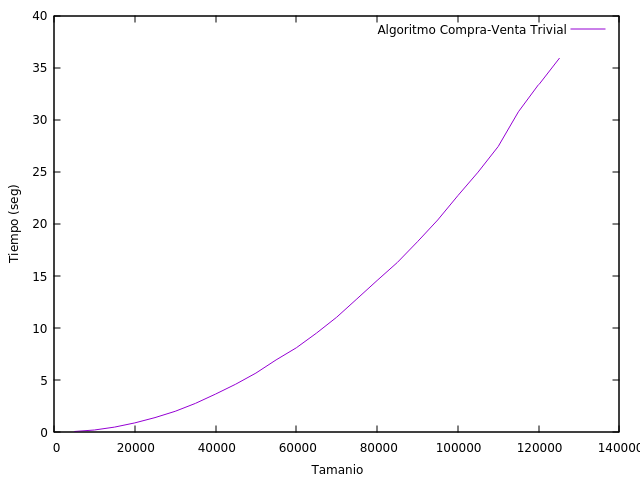
\includegraphics[scale = 0.8]{compraventatrivial.png}
\end{figure}
\subsection {Cálculo de la Eficiencia Híbrida}
La eficiencia híbrida calculada mediante gnuplot da como resultado el siguiente fichero  \\ \textcolor{ForestGreen}{\textbf{\code{fit\_trivial.log}}}:
\begin{minted}{text}
FIT:    data read from 'compraventatrivial.dat'
        format = z
        #datapoints = 25
        residuals are weighted equally (unit weight)

function used for fitting: f(x)
	f(x)=a0*x*x+a1*x+a2
fitted parameters initialized with current variable values

iter      chisq       delta/lim  lambda   a2            a1            a0           
   0 1.3487215210e+21   0.00e+00  4.24e+09    2.330664e-09  -4.438380e-06
   5 6.9420451076e-01  -4.96e-10  4.24e+04    2.330664e-09  -4.438380e-06

After 5 iterations the fit converged.
final sum of squares of residuals : 0.694205
rel. change during last iteration : -4.95775e-15

degrees of freedom    (FIT_NDF)                        : 22
rms of residuals      (FIT_STDFIT) = sqrt(WSSR/ndf)    : 0.177637
variance of residuals (reduced chisquare) = WSSR/ndf   : 0.0315548

Final set of parameters            Asymptotic Standard Error
=======================            ==========================
a2              = 2.33066e-09      +/- 0.1157       (4.965e+09%)
a1              = -4.43838e-06     +/- 4.102e-06    (92.41%)
a0              = 2.33066e-09      +/- 3.063e-11    (1.314%)

correlation matrix of the fit parameters:
                a2     a1     a0     
a2              1.000 
a1             -0.884  1.000 
a0              0.774 -0.971  1.000 
\end{minted}

De aquí concluimos que la formula ajustada es:

\[f(x)=\num{2.33066e-09}x² - \num{4.43838e-06}x + 2.33066e-09\]

Tras representar la función ajustada anterior en la gráfica de puntos podemos ver que se ajustan perfectamente:
\begin{figure}[H]
  \centering
  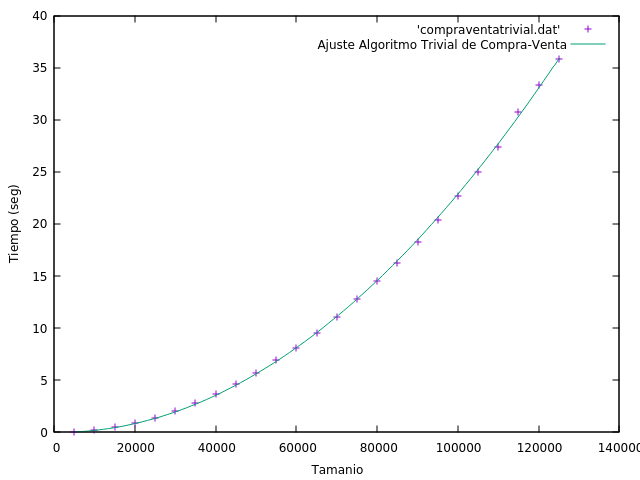
\includegraphics[scale = 0.8]{ajustecompraventatrivial.png}
\end{figure}

\section{Algoritmo basado en Divide y Vencerás}
La técnica de Divide y Vencerás nos permitirá pasar del algoritmo anterior una técnica muy ineficiente que tardaría mucho para grandes conjuntos de datos a un algoritmo mucho más eficiente. Para ello, en la implementación del Divide  y Vencerás, utilizamos la recursividad. 
\subsection{Implementación de la función de cómputo en C++ }


\begin{minted}{c++}
 int encontrarMinimo_izq(vector<int> &sentencia, int l, int r, int &dC){
	int minimo = sentencia[l];
	dC = l;
	for(int i = l; i <= r; i++)
		if(sentencia[i] < minimo){
			minimo = sentencia[i];
			dC= i;
		}
	return minimo;
}
\end{minted}

\begin{minted}{c++}
 int encontrarMaximo_der(vector<int> &sentencia, int l, int r, int &dV){
	int maximo = sentencia[l];
	dV=l;
	for( int i = l; i <= r; i++)
		if(sentencia[i] > maximo){
			maximo = sentencia[i];
			dV = i;
		}
	return maximo;
}
\end{minted}


\begin{minted}{c++}
int maxDiferencia(vector<int> &sentencia, int minimo, int maximo, int &dC,
                  int &dV){
  if (minimo>= maximo){
  	dC = dV = minimo;
  	return -9999;
  }
  int maxDiff = -99999, diaC, diaV;
  int mitad = (maximo + minimo) / 2;
  int izq_maxDiff = maxDiferencia(sentencia, minimo, mitad, dC, dV);
  diaC = dC;
  diaV = dV;
  int der_maxDiff = maxDiferencia(sentencia, mitad+1, maximo, dC, dV);
  if (izq_maxDiff > der_maxDiff){
  	maxDiff = izq_maxDiff;
  }else{
  	diaC = dC;
  	diaV = dV;
  	maxDiff = der_maxDiff;
  }
  int minimo_izq = encontrarMinimo_izq(sentencia, minimo, mitad, dC);
  int maximo_der = encontrarMaximo_der(sentencia, mitad + 1, maximo, dV);
  if ((maximo_der - minimo_izq) > maxDiff){
  	maxDiff = maximo_der - minimo_izq;
  	diaC = dC;
  	diaV = dV;
  }
  dC = diaC;
  dV = diaV;
  return maxDiff;
}
\end{minted}

\subsection{Cálculo de la Eficiencia teórica}

\begin{gather*}
  T(n) = I \cdot T(n/b) + G(n) = 2 \cdot T(\frac{n}{2}) + n \\
  I = 2^k = 2¹ \Rightarrow T(n) = O(n\log{n})
\end{gather*}

\[
  \begin{rcases*}
    I=2 \\
    b=2
    \end{rcases*}
  \
  \begin{tabular}{l}
     izq\_maxDiff = maxDiferencia(sentencia, minimo, mitad) \\
     der\_maxDiff = maxDiff = maxDiferencia(sentencia, mitad+1, maximo)
  \end{tabular}
\]

\[
 G(n) = D(n) + C(n) = O(1) + O(n) = O(n)
\]

\[
  \begin{rcases*}
    D(n) = 1
  \end{rcases*}
  mitad = \frac{maximo+minimo}{2}
\]

\[
  \begin{rcases*}
    \ \\
    C(n) = n \\
    \
    \end{rcases*}
  \
  \begin{tabular}{l}
  minima\_izq = encontrarMinimo\_izq(sentencia, minimo, mitad) \\
  maximo\_der = encontrarMaximo\_der(sentencia, mitad+1, maximo) \\
  maxDiff = max(izq\_maxDiff, der\_maxDiff, maximo\_der-minimo\_izq)
  \end{tabular}
\]

\subsection{Cálculo de la Eficiencia empírica}
\newpage

La tabla de datos resultante que obtenemos al ejecutarlo sin ningún optimizador de código es:
\begin{longtable}{|c|c|}
\hline
\textbf{Tamaño} & \textbf{Tiempo(seg)} \\ \hline
5000   & 0.00163401     \\ \hline
10000  & 0.000806976    \\ \hline
15000  & 0.00103244     \\ \hline
20000  & 0.00142681     \\ \hline
25000  & 0.00161177     \\ \hline
30000  & 0.00200034     \\ \hline
35000  & 0.00240804     \\ \hline
40000  & 0.00275965     \\ \hline
45000  & 0.00321197     \\ \hline
50000  & 0.00350924     \\ \hline
55000  & 0.00386887     \\ \hline
60000  & 0.00428708     \\ \hline
65000  & 0.00469606     \\ \hline
70000  & 0.00508064     \\ \hline
75000  & 0.00571565     \\ \hline
80000  & 0.00593092     \\ \hline
85000  & 0.0062978      \\ \hline
90000  & 0.00668497     \\ \hline
95000  & 0.0105791      \\ \hline
100000 & 0.00936575     \\ \hline
105000 & 0.0080948      \\ \hline
110000 & 0.0082681      \\ \hline
115000 & 0.00859129     \\ \hline
120000 & 0.00895775     \\ \hline
125000 & 0.0093908      \\ \hline
\end{longtable}


\newpage

Al usar gnuplot para graficar los datos anteriores, se crea la siguiente gráfica:
\begin{figure}[H]
  \centering
  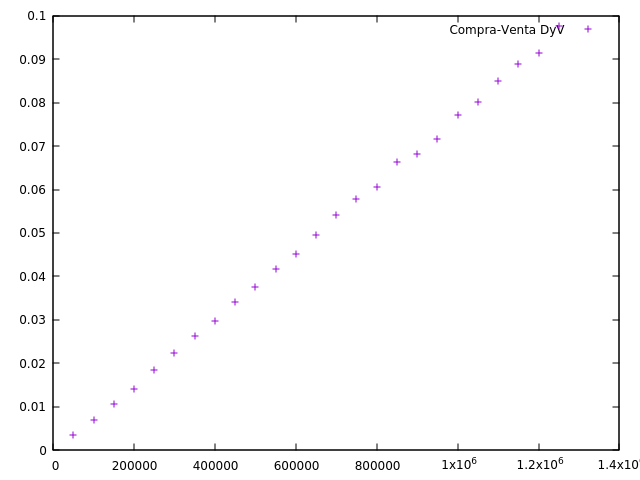
\includegraphics[scale = 0.8]{DyVwithpoints.png}
\end{figure}
\subsection{Cálculo de la Eficiencia Híbrida}

\begin{minted}{text}

FIT:    data read from 'compraventaDyV1.dat'
        format = z
        #datapoints = 25
        residuals are weighted equally (unit weight)

function used for fitting: f(x)
	f(x)=a*x*log(x)
fitted parameters initialized with current variable values

iter      chisq       delta/lim  lambda   a            
   0 2.6033979973e+15   0.00e+00  1.02e+07    1.000000e+00
   5 2.8801247962e-05  -2.24e-10  1.02e+02    5.580963e-09

After 5 iterations the fit converged.
final sum of squares of residuals : 2.88012e-05
rel. change during last iteration : -2.23513e-15

degrees of freedom    (FIT_NDF)                        : 24
rms of residuals      (FIT_STDFIT) = sqrt(WSSR/ndf)    : 0.00109547
variance of residuals (reduced chisquare) = WSSR/ndf   : 1.20005e-06

Final set of parameters            Asymptotic Standard Error
=======================            ==========================
a               = 5.58096e-09      +/- 2.147e-11    (0.3847%)
\end{minted}

La función ajustada que nos genera es:

\[f(x)=\num{5.58096e-09}xlog(x)\]

\newpage

Al ajustarla vemos que la función pasa por el medio de los puntos:
\begin{figure}[H]
  \centering
  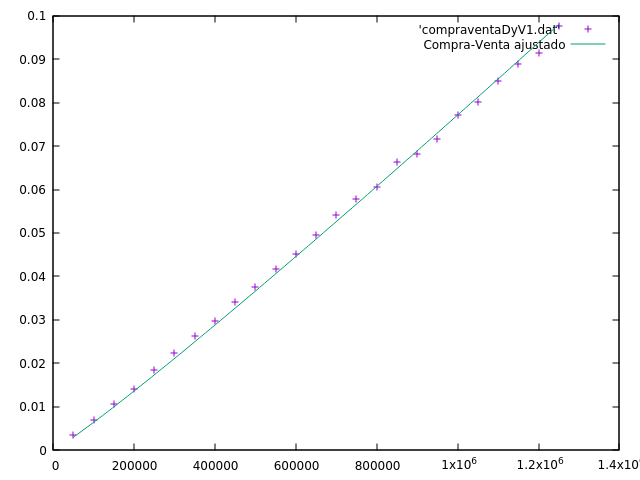
\includegraphics[scale = 0.8]{ajusteDyV.png}
\end{figure}

\vspace{5cm}
 \bibliographystyle{plain}
 \bibliography{biblist}


\end{document}
